\documentclass{article}
\usepackage{hyperref}
\usepackage[margin=1in]{geometry}
\usepackage{indentfirst}   % Indents first paragraph. change if u want ig
\usepackage{setspace} 
\doublespacing
\usepackage{graphicx}
\graphicspath{ {images_arch} }
\usepackage{listings}
\usepackage{xcolor}
\lstset{
  basicstyle=\ttfamily,
  columns=fullflexible,
  breaklines=true,
  postbreak=\raisebox{0ex}[0ex][0ex]{\color{red}$\hookrightarrow$\space}
}

\begin{document}
\title{\textbf{Final Undergraduate Psuedo-Sudoku Submission}}
\author{Spencer Hirsch, Thomas Johnson}
\date{\today}

\maketitle

\noindent \textbf{Summary of Project}

\medskip

Following our original submission we have implemented another algorithm. With 
our original submission we implemented a backtracking algorithm, which worked
very well for our first milestone. For this final milestone we have implemented
a backtracking with a heuristic algorithm. Both algorithms solve the given
test cases, however after doing an analysis of the two comparing the input size and
the number of removed cells there is a clear difference in the complexity of the
two different algorithms. 

In order to generate reasonable test cases to demonstrate the time complexity of our
our two algorithms. We have implemented a generator to generate test cases to give to
our algorithms. Each algorithm tests a total of 2700 different test cases with varying
difficulty. The goal of implementing a generator was to make the tests as random as 
possible and to easily generate a larger sum of test cases. For each n (the size of 
the matrix, n x n) there are 15 additional test cases that have varying m (number of 
missing cells). Each of these n x m combinations is tested a total of 30 times. This 
is how we have determined that there are a total of 2700 different test cases run on
each of the algorithms. 

All aspects of the board aside from the size of the board is randomly determined. The 
values for each squares are randomly assigned for the size of the board. Once all of
the values are determined the number of removed cells is randomly selected and unique 
to each row. The purpose of creating this random algorithm was to ensure that bias was 
reduced. 

In order to demonstrate the time complexity of each of the algorithms the cpu time is
recorded for each test and plotted against the number of removed squares from the sudoku
board. To ensure the accuracy of our results the same test cases are run on both of the
algorithms. Two scatter plots are constructed for the two algorithms, one displaying every
point gathered from the test sets and the other plot demonstrating the averages of the 15
ponints for each n x m pair. 

\pagebreak

\noindent \textbf{Backtracking Algorithm}

\begin{lstlisting}[frame=single]
	# Function next empty cell in the matrix
	
	def find_cell(board, size):
		iterate through the board to find the next instance of a 0 value in
		a cell
	
		If no value is found, return -1, -1
	
		otherwise return the coordinate of the cell that contains a 0 value	
	
	
	# Function checks for a valid move given the value of the current
	# Cell
	
	def valid_move(coordinate_1, coordinate_2, board, size, number):
	
		Iterate through the size of the board
			Check to see if there is a cell in the column has the current val
				if so, return false
	
		Iterate through the size of the board
			Check to see if there is a cell in the row that has the current val
				If so, return false
	
		return true  # It is a valid move for the algorithm to make
	
	
	def solve(board, size):
		Create a list of all possible numbers based on size of the board
		Find the coordinate to the next empty cell
		
		Check to see if cell is valid
	
		iterate through all possible numbers to fill a cell
			Check to see if the move is a vlid move
		
		Continue until all cells are filled or no solution is found
\end{lstlisting}

\textit{How the backtracking algorithm works:} \\

\pagebreak

\noindent \textbf{Backtracking with Heuristic}


\textit{How the backtracking with heuristic algorithm works}: \\


\pagebreak

\noindent \textbf{Analysis of Algorithms}



\noindent \textit{Backtracking} \\ \\
% Change the images
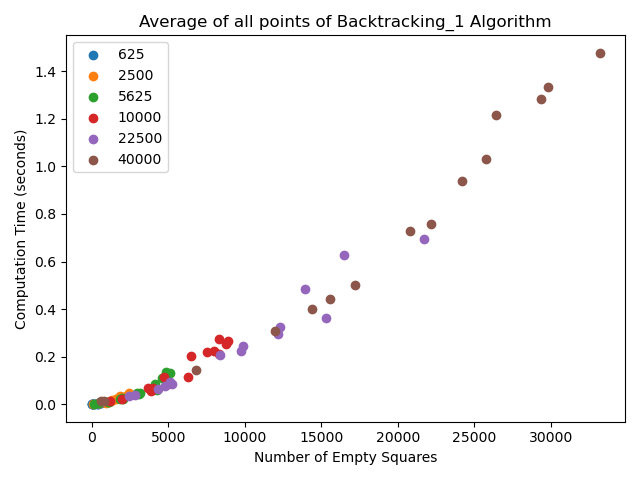
\includegraphics[scale=0.5]{scatter_avg_Backtracking_1-1.png}
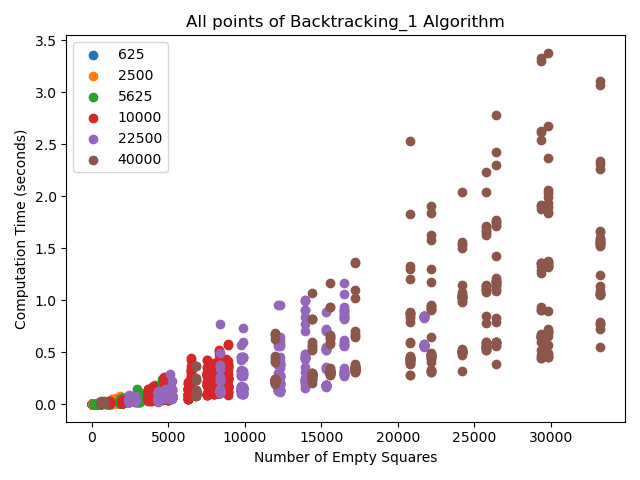
\includegraphics[scale=0.5]{scatter_Backtracking_1-1.png}

\bigskip

\noindent \textit{Backtracking with Heuristic} \\ \\
% Change the images
\includegraphics[scale=0.5]{scatter_avg_Backtracking_w_Heuristic-1.png}
\includegraphics[scale=0.5]{scatter_Backtracking_w_Heuristic-1.png}


From the images it is clear to see that there is a significant difference in
time complexity between the backtracking algorithm and the forward-checking 
with heuristic algorithm. The graph with the average of the points of the
backtracking shows what we believe to be O($n^2$) for time complexity. As the
number of missing cells increases there appears to be an exponential growth
with respect to time. However, in the case of the backtracking algorithm with
a heuristic, it is much more difficult to determine Big-Oh complexity. In this 
specific test case it appears to loosely conform to O(logn) complexity. However,
strictly looking at the y-axis on both of the graphs we can see that the backtracking 
with heuristic algorithm performs much quicker than the previous backtracking algorithm.

\bigskip

Here are some additional examples with some other test cases.

\noindent \textit{Backtracking} \\ \\
% Change the images
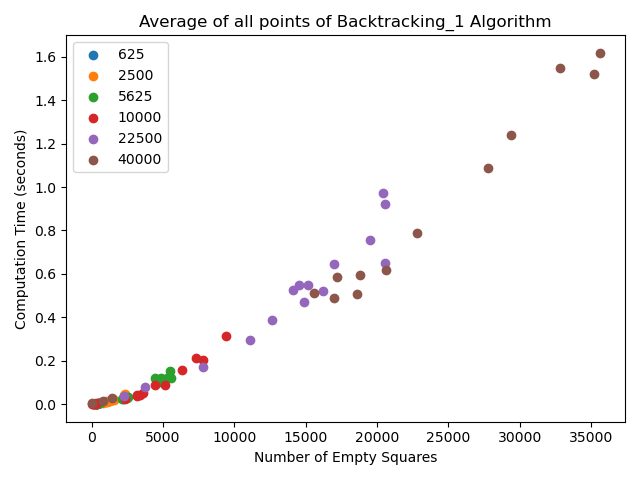
\includegraphics[scale=0.5]{scatter_avg_Backtracking_1-2.png}
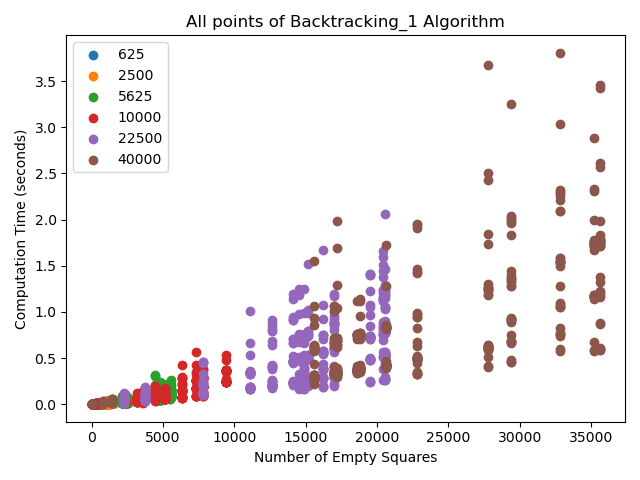
\includegraphics[scale=0.5]{scatter_Backtracking_1-2.png}

\bigskip

\noindent \textit{Backtracking with Heuristic} \\ \\
% Change the images
\includegraphics[scale=0.5]{scatter_avg_Backtracking_w_Heuristic-2.png}
\includegraphics[scale=0.5]{scatter_Backtracking_w_Heuristic-2.png}

Again, with this test case the backtracking algorithm appears to be in the shape of O($n^2$).
However, the backtracking algorithm with heuristic appears to be more in the shape of constant
time, besides the single point which is clearly an outliar. Despite the drastic change in the 
shape of the graph for the backtracking with heuristic algorithm, the backtracking with heuristic algorithm
performs much quicker than the backtracking algorithm that was originally implemented.

\bigskip

\noindent \textit{Backtracking} \\ \\
% Change the images
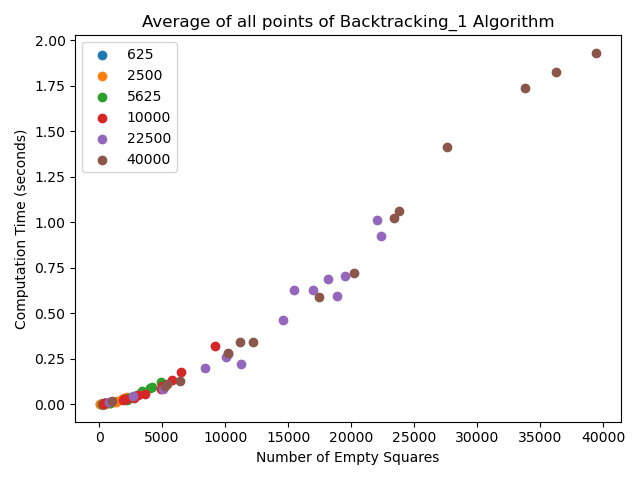
\includegraphics[scale=0.5]{scatter_avg_Backtracking_1-3.png}
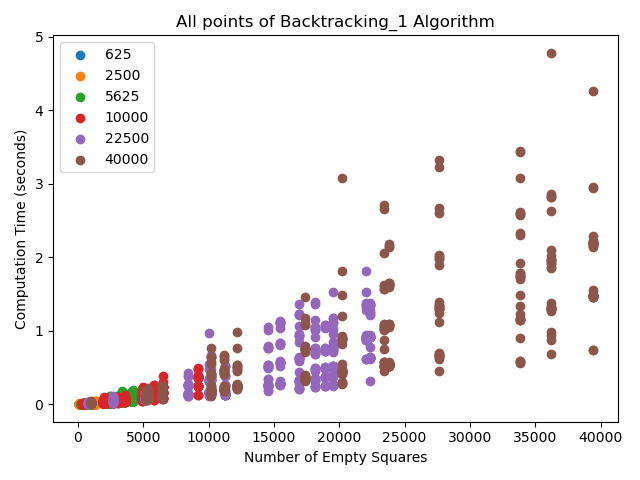
\includegraphics[scale=0.5]{scatter_Backtracking_1-3.png}

\bigskip

\noindent \textit{Backtracking with Heuristic} \\ \\
% Change the images
\includegraphics[scale=0.5]{scatter_avg_Backtracking_w_Heuristic-3.png}
\includegraphics[scale=0.5]{scatter_Backtracking_w_Heuristic-3.png}

These test cases aligned more with the first test case listed above. The
backtracking algorithm again having more of a O($n^2$) complexity while the
backtracking with heuristic algorithm had more of a O(logn) shape. Again, 
the averages of the tests showed that the backtracking algorithm with heuristic
signigicantly outperformed the backtracking algorihtm that was originally used.


% \pagebreak

% \textbf{Summary of the intermediate submission:}

% \bigskip

% \noindent For this assignment, my partner and I used the backtracking algorithm in order
% to solve for the problem. Our program reads in a text file that conatins the 
% number of rows and columns as well as a list of the values that the matrix will
% be made up of. The values will be read in by row,

% \[R_{00},R_{01},R_{02},R_{03},R_{10},R_{11},R_{12},R_{13},R_{20},R_{21},R_{22},R_{23},R_{30},R_{31},R_{32},R_{33}\]

% \noindent The values are then placed in their repsective places in the n $\times$ n matrix.
% The initial empty spaces hold a value of 0, the algorithm will search for the 0's 
% in the matrix and replace them with their correct value. We chose to use a backtracking
% algorithm in order to solve this problem. The psuedo-code for our solution is posted above.
% The solution that we came to is our original code.

\end{document}